% 建议使用 XeLaTeX 或 LuaLaTeX 编译(更佳的中文支持)
\documentclass[UTF8,zihao=-4]{ctexart}

% 统一导言
\usepackage[a4paper,margin=2.5cm]{geometry}
\usepackage{amsmath,amssymb,amsthm}
\usepackage{bm}
\usepackage{hyperref}
\usepackage{graphicx}
\usepackage{caption}
\usepackage{listings}
\usepackage{xcolor}
\usepackage{float}
\usepackage{placeins}

% 图片路径
\graphicspath{{figures/}}

% 统一代码风格
\lstdefinestyle{code}{%
  language=Python,
  basicstyle=\ttfamily\small,
  numbers=left,
  numberstyle=\tiny,
  keywordstyle=\color{blue}\bfseries,
  commentstyle=\color{teal!70!black},
  stringstyle=\color{orange!70!black},
  breaklines=true,
  frame=single,
  rulecolor=\color{black!30},
  tabsize=2,
  showstringspaces=false
}
\lstset{style=code}

\title{支持向量机(SVM):理论与实践}
\author{}
\date{\today}

\begin{document}
\maketitle

% 结构:Introduction / Theory and Formulas / Applications and Tips / Python Practice / Result / Summary

\section{引言}
支持向量机(SVM)属于基于间隔(margin)的判别式模型,通过最大化类间间隔来提升泛化能力。引入核函数(kernel)后,可在保持凸优化性质的同时刻画复杂的非线性决策边界。

\section{原理与公式}
以线性、软间隔 SVM 的原始问题为例,给定标注数据 $\{(\mathbf{x}_i, y_i)\}_{i=1}^n$,$y_i\in\{-1,+1\}$:
\begin{align}
\min_{\mathbf{w}, b, \boldsymbol{\xi} \ge 0} \quad & \tfrac{1}{2}\lVert \mathbf{w} \rVert^2 + C \sum_{i=1}^n \xi_i \\
\text{s.t.} \quad & y_i (\mathbf{w}^\top \mathbf{x}_i + b) \ge 1 - \xi_i,\; i=1,\dots,n.
\end{align}
对偶形式仅依赖于内积,将其替换为核函数 $K(\mathbf{x},\mathbf{x}')$ 即得非线性 SVM。决策函数为:
\begin{equation}
f(\mathbf{x}) = \sum_{i \in SV} \alpha_i y_i K(\mathbf{x}_i, \mathbf{x}) + b, \quad \hat{y} = \mathrm{sign}\, f(\mathbf{x}),
\end{equation}
其中 $SV$ 为支持向量($\alpha_i>0$)。常用的 RBF 核为 $K(\mathbf{x},\mathbf{x}')=\exp(-\gamma\lVert\mathbf{x}-\mathbf{x}'\rVert^2)$。超参数 $C$ 控制软间隔惩罚,$\gamma$ 控制边界复杂度。

\section{应用与技巧}
\begin{itemize}
  \item \textbf{缩放:} 必须进行特征缩放;SVM 对尺度高度敏感。
  \item \textbf{调参:} 通过交叉验证选择 $C$ 与(RBF 的)$\gamma$;可从对数网格开始(例如 $C\in[0.1,10]$、$\gamma\in[10^{-2},10]$)。
  \item \textbf{类不平衡:} 使用 \texttt{class\_weight=balanced} 进行重加权。
  \item \textbf{概率输出:} 在 \texttt{SVC} 中设 \texttt{probability=True} 可获得概率(需额外校准开销);否则使用 \texttt{decision\_function}。
  \item \textbf{多分类:} \texttt{SVC} 采用一对一策略;\texttt{LinearSVC} 采用一对其余。
\end{itemize}

\section{Python 实战}
在本章节目录运行下述命令,图片将保存到 \texttt{figures/}:
\begin{lstlisting}[style=code,caption={生成 SVM 配图},label={lst:genfigs_svm_cn}]
python gen_svm_figures.py
\end{lstlisting}

% 纳入完整 Python 源码
\lstinputlisting[style=code,caption={gen\_svm\_figures.py 源码},label={lst:source_svm_cn}]{gen_svm_figures.py}

\section{结果}
\begin{figure}[H]
  \centering
  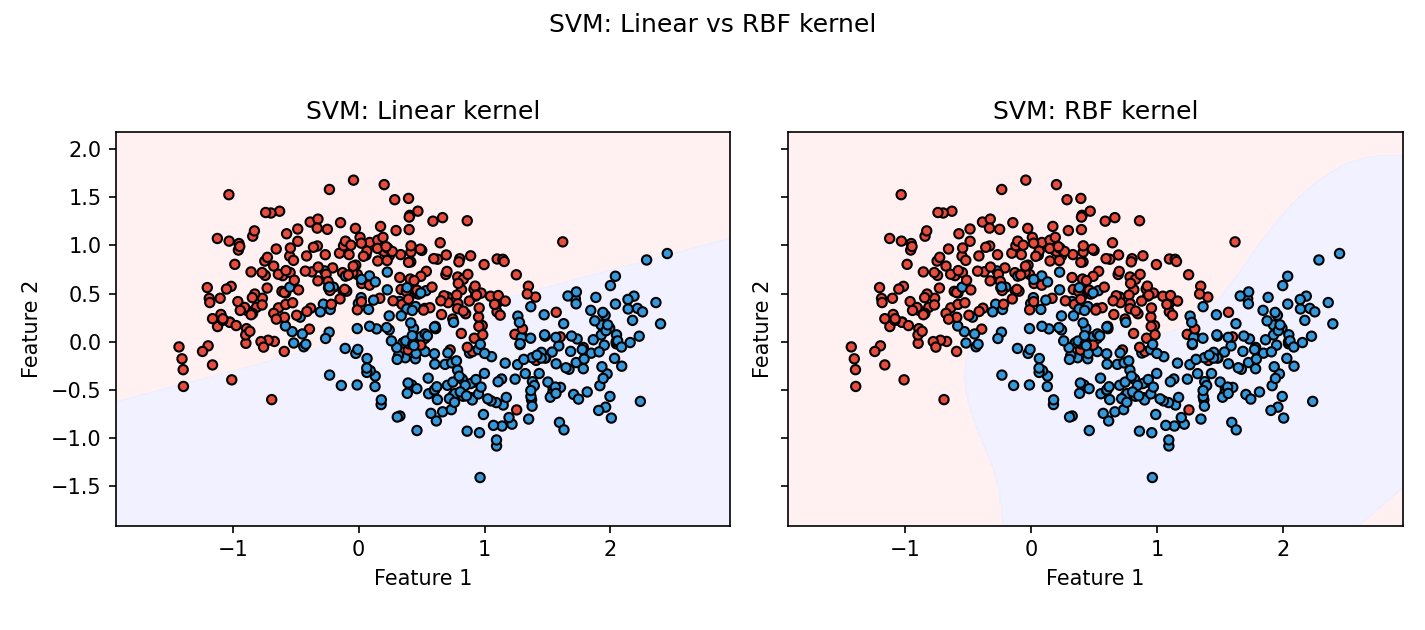
\includegraphics[width=0.95\linewidth]{svm_linear_vs_rbf.png}
  \caption{SVM 决策边界:线性核 vs RBF 核。}
  \label{fig:svm_lin_rbf_cn}
\end{figure}
\FloatBarrier

\begin{figure}[H]
  \centering
  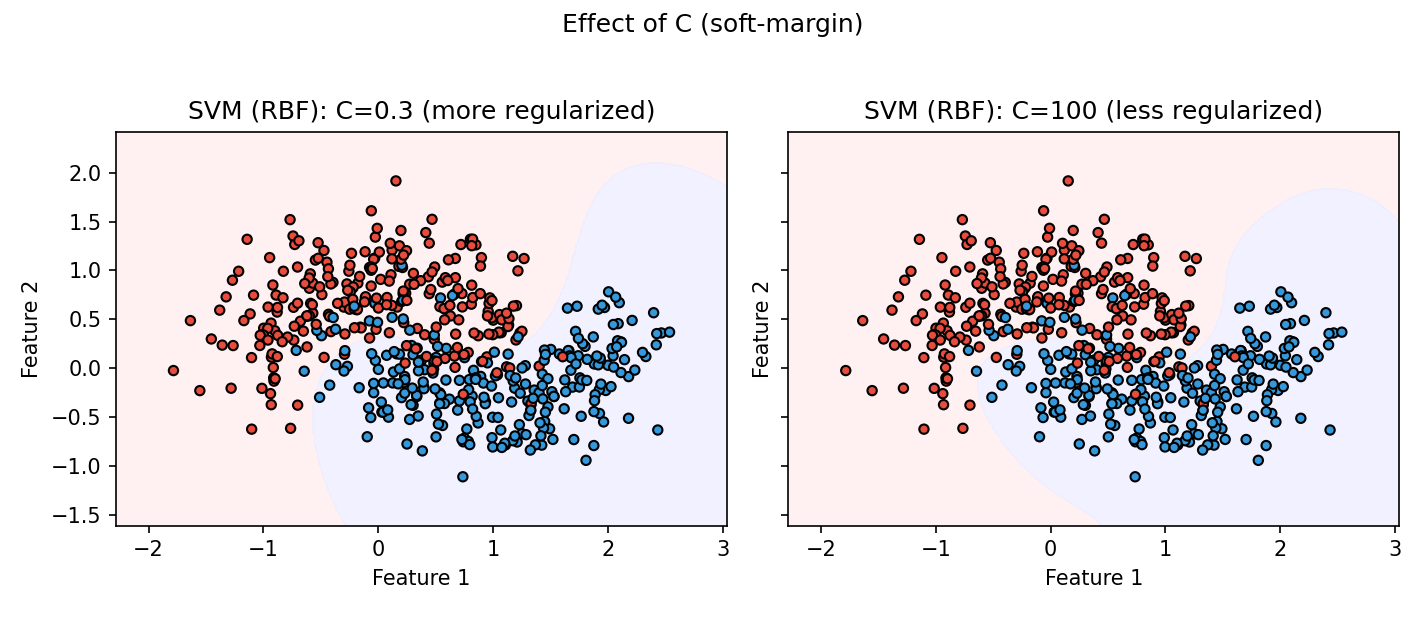
\includegraphics[width=0.95\linewidth]{svm_C_compare.png}
  \caption{软间隔参数 C 的影响(RBF 核)。}
  \label{fig:svm_c_cn}
\end{figure}
\FloatBarrier

\begin{figure}[H]
  \centering
  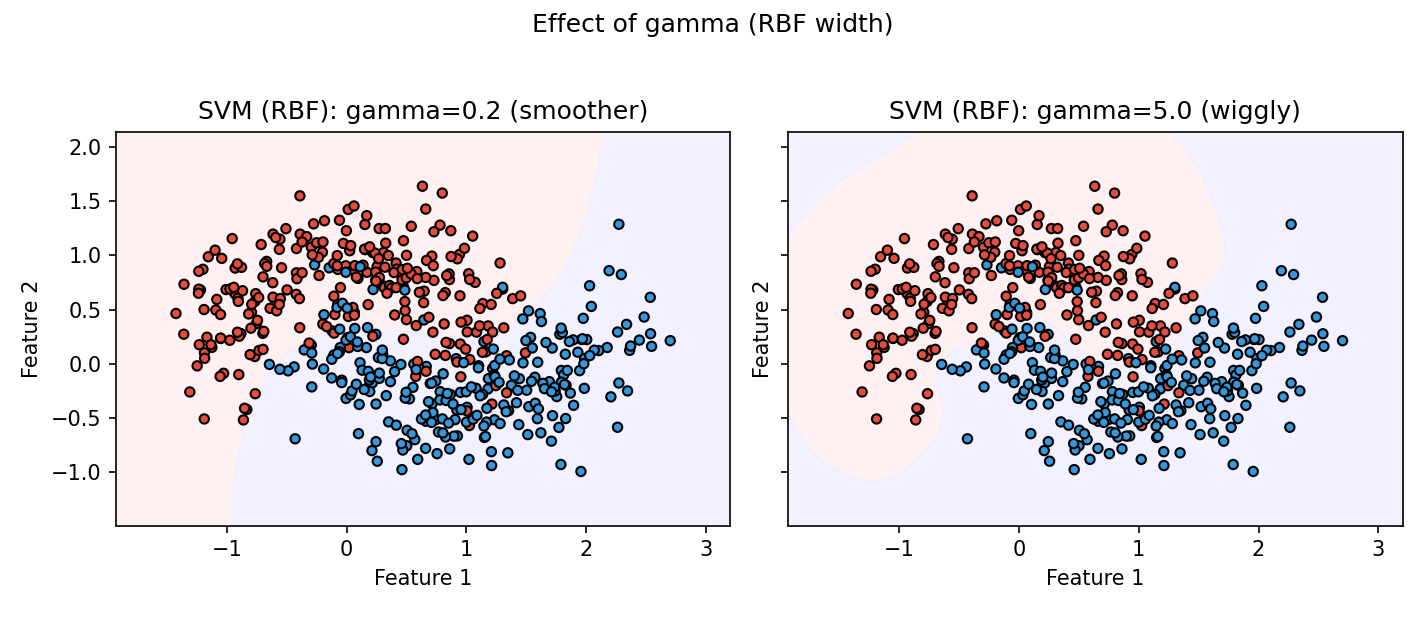
\includegraphics[width=0.95\linewidth]{svm_gamma_compare.png}
  \caption{RBF 的 $\gamma$ 对边界平滑度的影响。}
  \label{fig:svm_gamma_cn}
\end{figure}
\FloatBarrier

\begin{figure}[H]
  \centering
  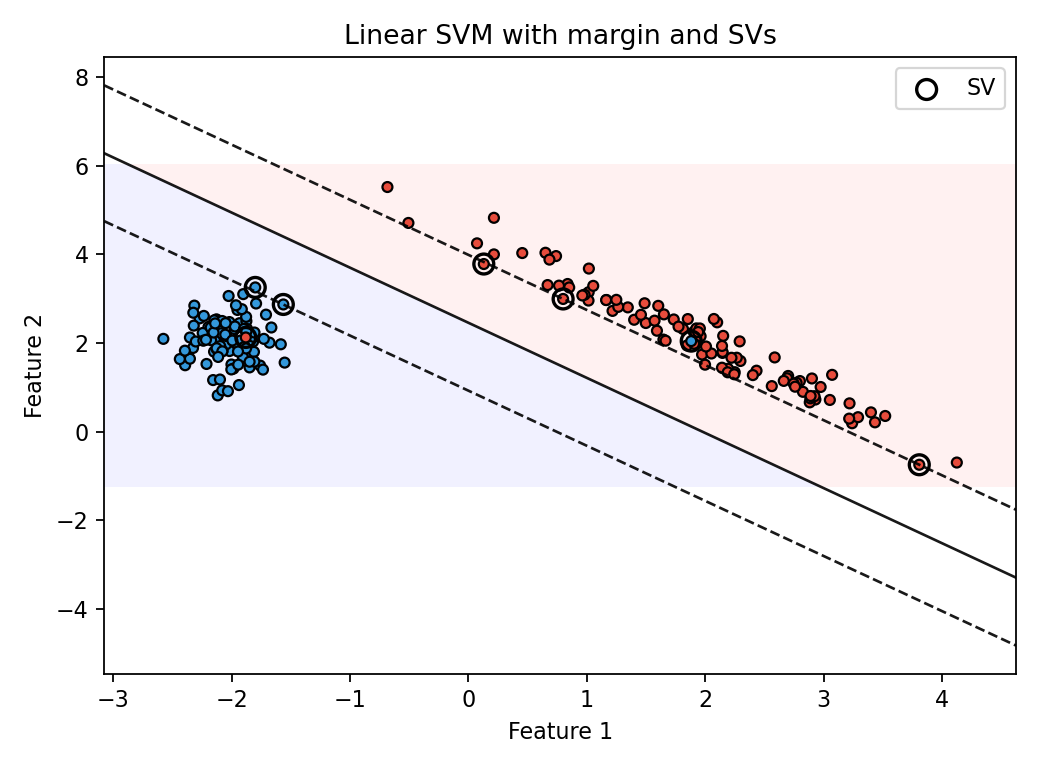
\includegraphics[width=0.85\linewidth]{svm_margin_support_vectors.png}
  \caption{线性 SVM:间隔线与支持向量可视化。}
  \label{fig:svm_margin_cn}
\end{figure}
\FloatBarrier

\begin{figure}[H]
  \centering
  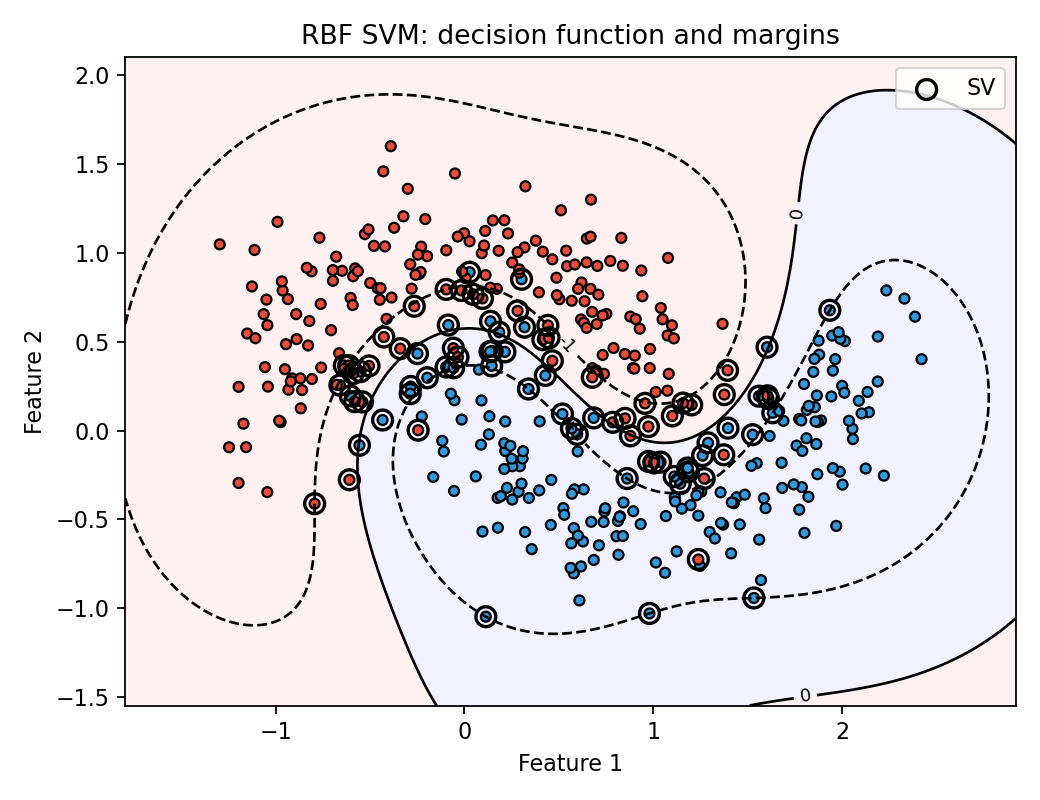
\includegraphics[width=0.85\linewidth]{svm_decision_function.png}
  \caption{RBF SVM 的决策函数:-1、0、+1 等值线。}
  \label{fig:svm_df_cn}
\end{figure}
\FloatBarrier

\section{总结}
SVM 通过最大化间隔实现稳健分类,并可借助核函数处理非线性问题。在恰当的特征缩放与 $C$、核参数的调参与验证下,SVM 常在多种任务上表现优异。

\end{document}

